\chapter{Pulbangash Metro Station}

\section{Station Design and Overview}
\par\noindent
Pulbangash is an underground metro station being constructed as part of the Delhi Metro Phase IV network under Contract DC-05, CPM-3. The station lies along the corridor connecting Janakpuri West to RK Ashram, situated beneath the densely populated and historically significant area of Sadar Bazar in Old Delhi. The station is designed to serve as a critical node handling high passenger footfall from the surrounding commercial and residential areas.

\par\noindent
Underground metro stations of this scale are far more complex to design and build than elevated stations. The station box must be excavated deep into the ground while simultaneously supporting the surrounding soil, existing utilities, and overlying structures. At Pulbangash, this challenge is compounded by the dense urban fabric above ground, with narrow roads, old buildings of uncertain foundation quality, and a high water table typical of Delhi's alluvial subsoil.

\par\noindent
The station follows DMRC's standard underground station typology with a concourse level above the platform level, connected by staircases, escalators, and lifts. The platform is of the island type, with tracks running on both sides.

\begin{figure}[ht]
    \centering
    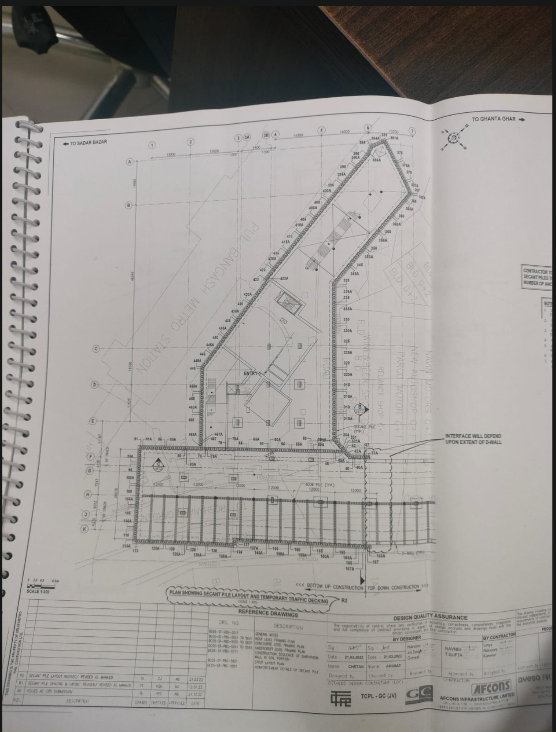
\includegraphics[width=0.85\textwidth]{content/images/station_plan.png}
    \caption{Plan layout of Pulbangash station showing the overall footprint, D-Wall perimeter, and tunnel alignment}
    \label{fig:station_plan}
\end{figure}

\section{Site Visit}
\par\noindent
The site visit to Pulbangash station provided direct exposure to an active underground metro construction site at an intermediate stage. The diaphragm wall had already been constructed forming the perimeter retaining structure, and excavation of the station box was underway with strutting systems visible at multiple levels, as seen in Figure \ref{fig:station_box_overview}. Workers and machinery were operating within the excavation, and the scale of the operation vividly illustrated the engineering involved in building underground infrastructure in a dense urban environment.

\section{Platform Outside the Main Box --- Sadar Bazar}
\par\noindent
One of the most distinctive engineering features at Pulbangash is that the platform extends outside the main station box. In a conventional underground station, the entire platform is contained within the main station box. At Sadar Bazar/Pulbangash however, the alignment geometry and the surface constraints meant that the full platform length could not be accommodated within a single rectangular box without demolishing a disproportionate number of structures above ground.

\par\noindent
The solution adopted was to extend the platform tunnel beyond one end of the main box, so that part of the platform sits within the bored tunnel section rather than the cut-and-cover box. This means the TBM-bored tunnel transitions directly into the station platform at one end. This arrangement has significant implications for the structural design, waterproofing strategy, and fit-out, as the junction between the circular tunnel lining and the rectangular box must be carefully detailed to handle differential settlement and waterproofing continuity across the geometric transition.

\section{Construction Method}
\par\noindent
The main station box is being constructed using the bottom-up Cut and Cover method. The perimeter Diaphragm Wall, constructed before excavation, serves as both the temporary earth retaining structure and the permanent station wall. At certain locations, secant pile walls are used where D-Wall construction is geometrically impractical. Detailed discussion of these construction methods and the concrete specifications used have been covered in the Batching Plant and Casting Yard chapter.

\begin{figure}[ht]
    \centering
    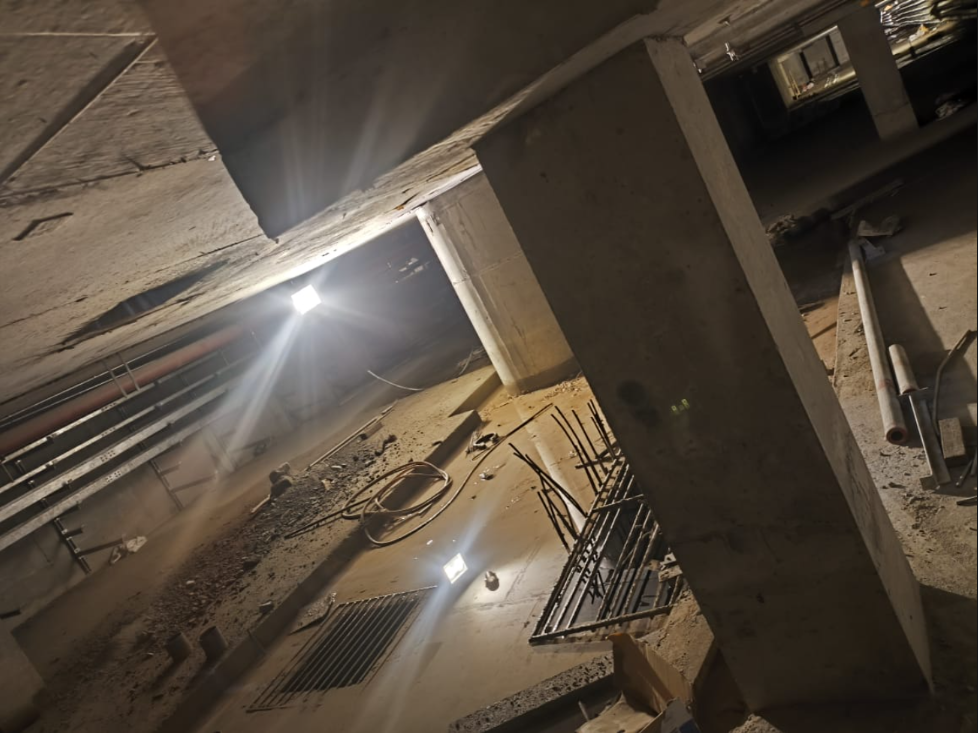
\includegraphics[width=0.85\textwidth]{content/images/station_box_interior.png}
    \caption{Interior of the station box under construction showing completed concrete columns and roof slab}
    \label{fig:station_box_overview}
\end{figure}

\subsection{Secant Pile Wall}
\par\noindent
A secant pile wall consists of interlocking bored piles --- alternating hard piles (reinforced) and soft piles (unreinforced) --- where the hard piles cut into the soft piles to create a continuous interlocked retaining wall. The reinforcement configurations vary at each strut level depending on the depth and lateral pressures to be resisted, as shown in the reinforcement drawings in Figure \ref{fig:secant_pile_drawing}.

\begin{figure}[ht]
    \centering
    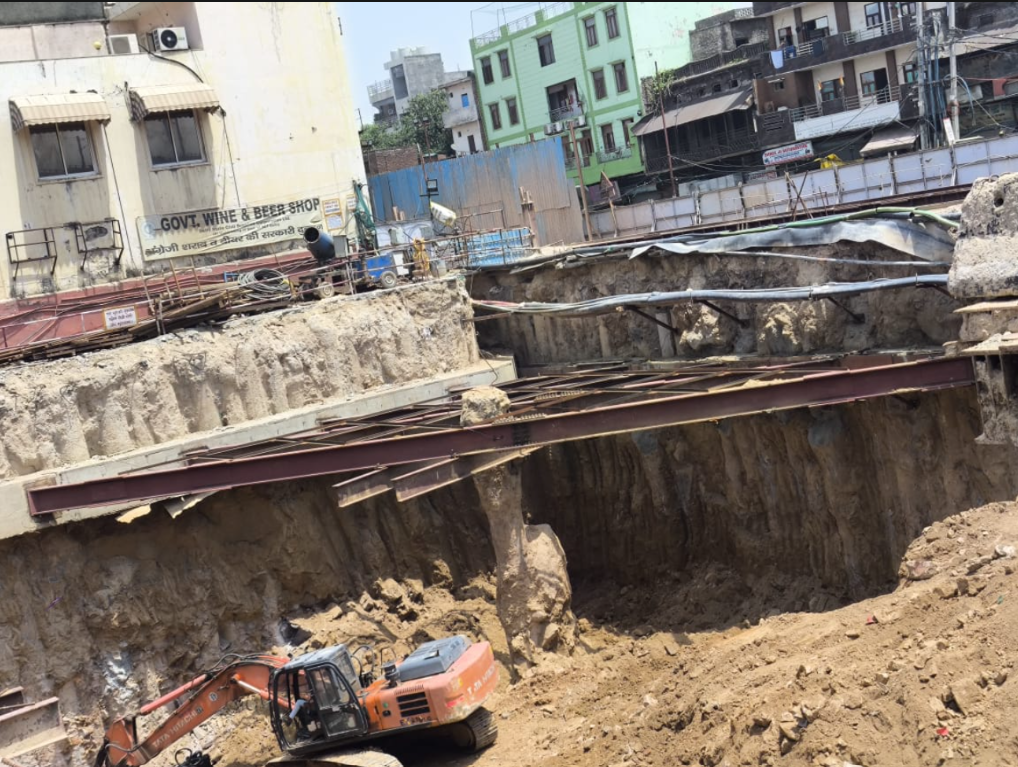
\includegraphics[width=0.8\textwidth]{content/images/secant_pile_exposed.png}
    \caption{Exposed face of the secant pile wall at Pulbangash showing the interlocking hard and soft pile pattern}
    \label{fig:secant_pile_exposed}
\end{figure}

\begin{figure}[ht]
    \centering
    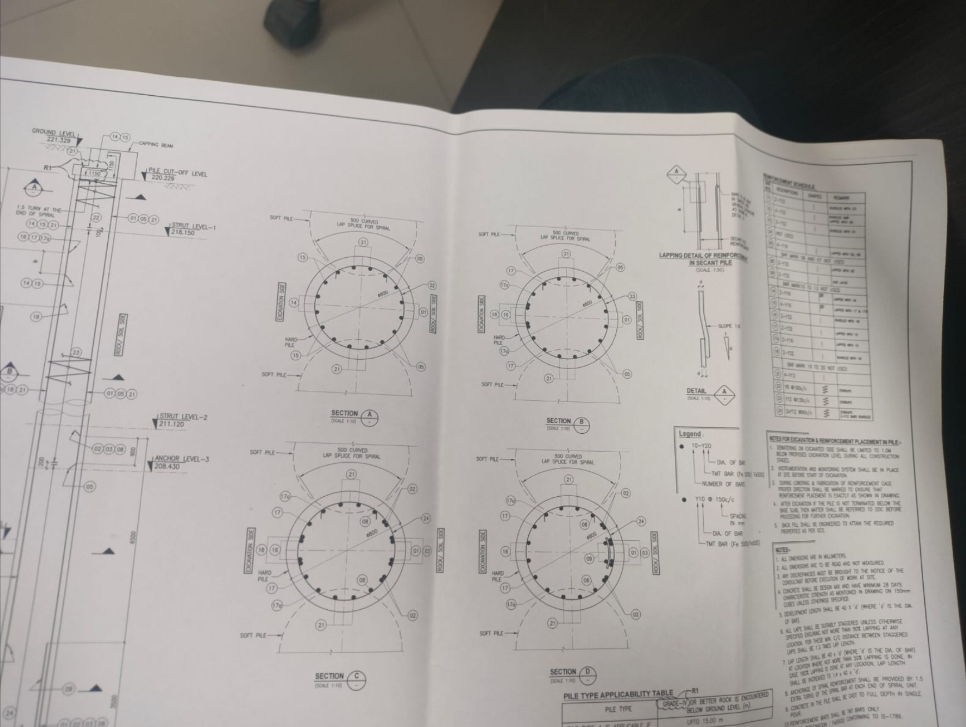
\includegraphics[width=0.85\textwidth]{content/images/secant_pile_drawing.png}
    \caption{Reinforcement detail drawing of the secant pile wall showing cross-sections at different strut levels}
    \label{fig:secant_pile_drawing}
\end{figure}

\subsection{Pile Cage Installation --- Staged Methodology}
\par\noindent
The installation of the pile cage for secant piles follows a carefully staged eight-step procedure to ensure the cage is correctly positioned within the bored hole. The methodology is necessitated by the length of the pile cage, which makes it impossible to simply lift it vertically from a horizontal position in a single motion. The gradual rotation minimises dynamic loading on the cage and ensures it enters the bore hole cleanly.

\par\noindent
\textbf{Stage 1:} The piling rig is positioned at a 5.5 m radius away from the pile cage location. The pile cage, 12 m in length, is held vertically alongside the rig at ground level, as shown in Figure \ref{fig:pile_stage1}.

\begin{figure}[ht]
    \centering
    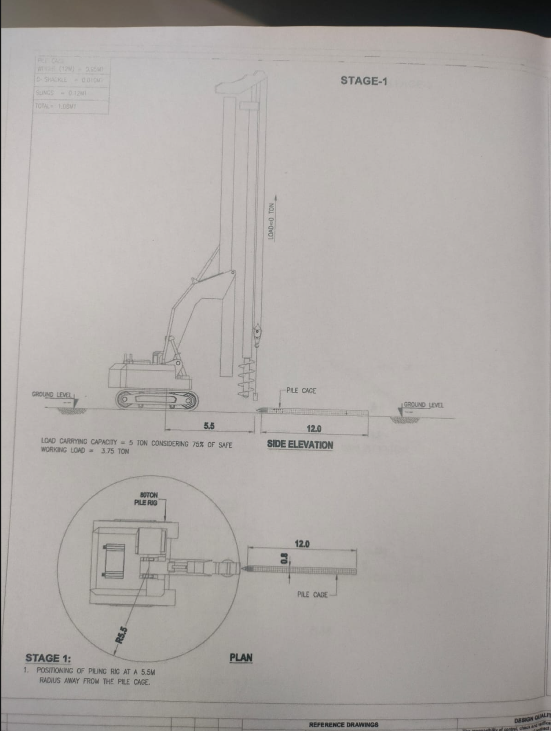
\includegraphics[width=0.75\textwidth]{content/images/pile_stage1.png}
    \caption{Stage 1 --- Piling rig positioned at 5.5 m radius with pile cage held at ground level}
    \label{fig:pile_stage1}
\end{figure}

\par\noindent
\textbf{Stage 2:} The rig begins gradually lifting the cage, tilting it from vertical toward the bore hole.

\par\noindent
\textbf{Stage 3:} The cage is lifted to 30\textdegree\ from horizontal.

\par\noindent
\textbf{Stage 4:} The cage reaches 45\textdegree\ from horizontal, as shown in Figure \ref{fig:pile_stage4}.

\begin{figure}[ht]
    \centering
    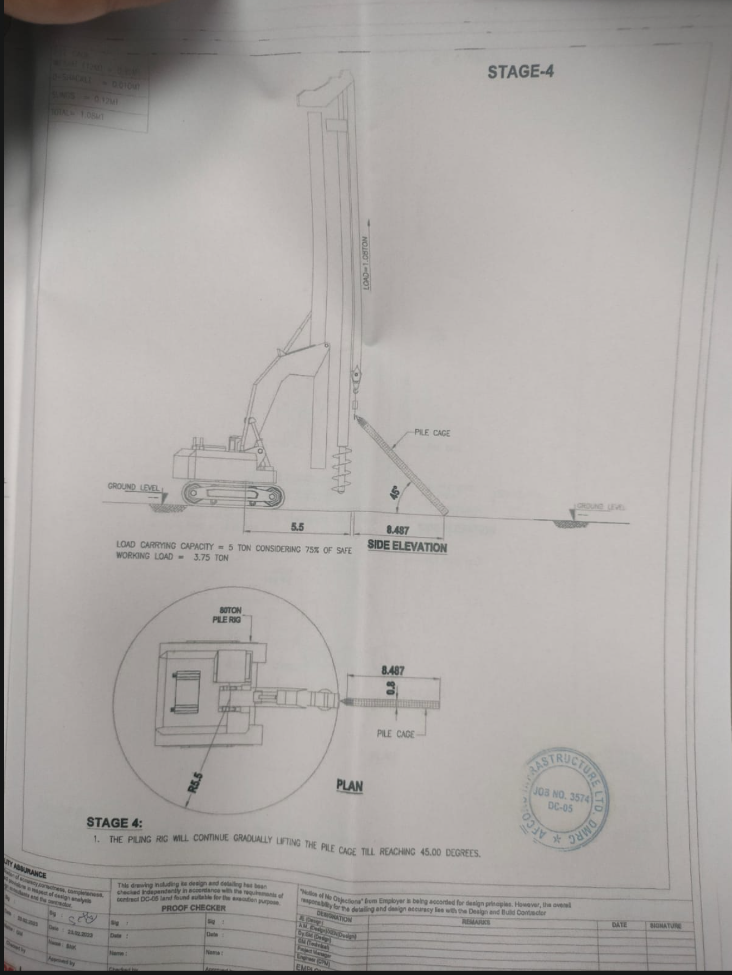
\includegraphics[width=0.75\textwidth]{content/images/pile_stage4.png}
    \caption{Stage 4 --- Pile cage lifted to 45\textdegree\ from horizontal while maintaining the same angle and length}
    \label{fig:pile_stage4}
\end{figure}

\par\noindent
\textbf{Stage 5:} The cage reaches 60\textdegree\ from horizontal.

\par\noindent
\textbf{Stage 6:} The cage reaches 80--90\textdegree, positioned directly over the bore hole.

\par\noindent
\textbf{Stage 7:} With the cage now near-vertical and aligned over the bore hole, the rig begins lowering it slowly into the trench, as shown in Figure \ref{fig:pile_stage7}.

\begin{figure}[ht]
    \centering
    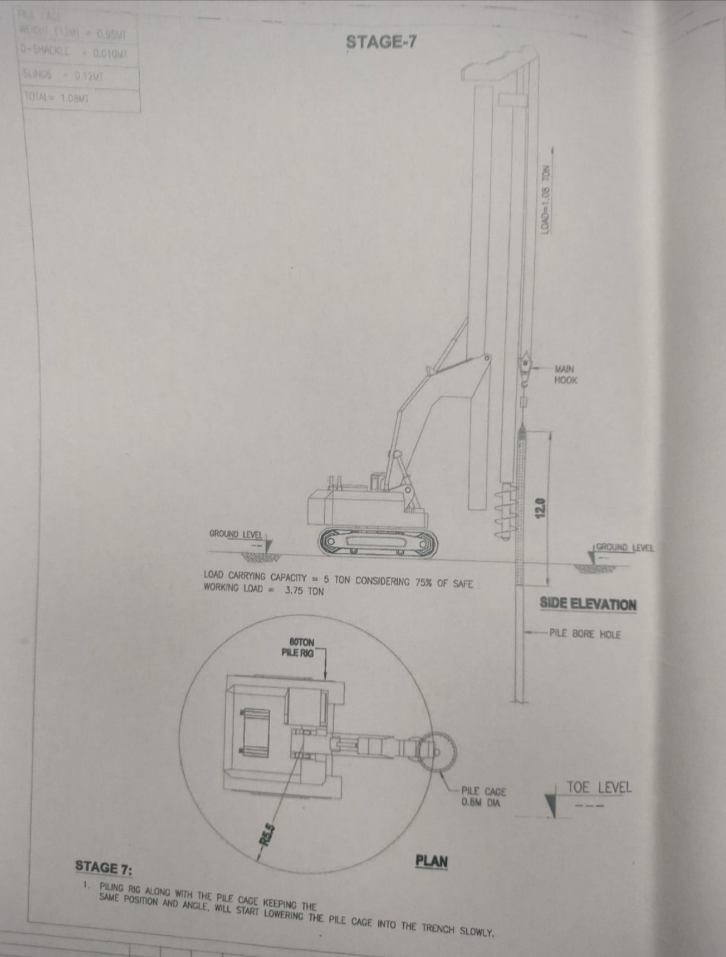
\includegraphics[width=0.75\textwidth]{content/images/pile_stage7.png}
    \caption{Stage 7 --- Cage now vertical, being slowly lowered into the pile bore hole}
    \label{fig:pile_stage7}
\end{figure}

\par\noindent
\textbf{Stage 8:} Once lowered to the required depth, the cage is rested on a resting beam at the correct level before concreting begins, as shown in Figure \ref{fig:pile_stage8}.

\begin{figure}[ht]
    \centering
    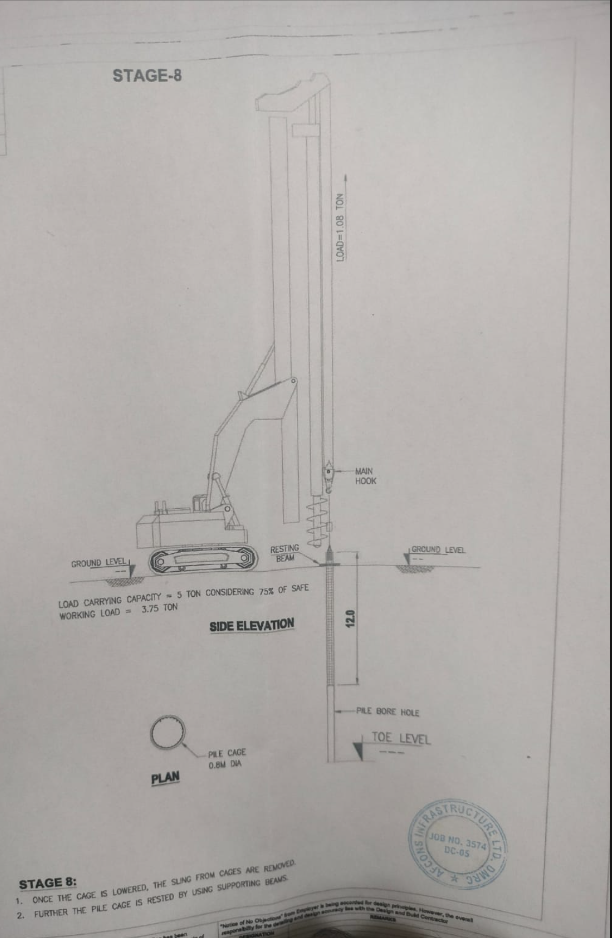
\includegraphics[width=0.75\textwidth]{content/images/pile_stage8.png}
    \caption{Stage 8 --- Cage fully lowered and rested on supporting beam, ready for concreting}
    \label{fig:pile_stage8}
\end{figure}

\subsection{Strutting System}
\par\noindent
As excavation progresses downward, the D-Wall panels face increasing lateral earth and water pressure. To prevent inward deflection, a temporary strutting system is installed at multiple levels. The struts are steel sections spanning across the excavation from wall to wall, installed at each level before excavation proceeds below it. At Pulbangash, three support levels were provided --- Strut Level-1 at approximately 218.150 m, Strut Level-2 at 211.120 m, and Anchor Level-3 at 208.430 m.

\begin{figure}[ht]
    \centering
    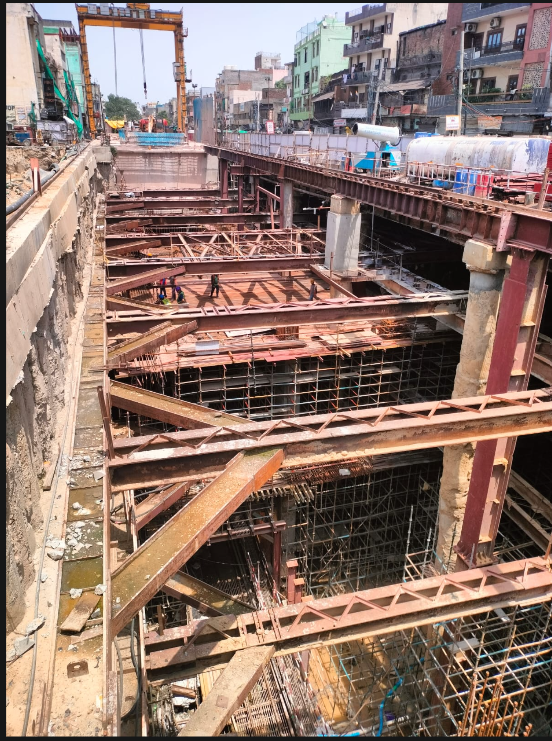
\includegraphics[width=0.85\textwidth]{content/images/station_box_struts.png}
    \caption{Open station box excavation viewed from above showing multiple levels of steel struts spanning the full width of the excavation}
    \label{fig:station_box_struts}
\end{figure}

\begin{figure}[ht]
    \centering
    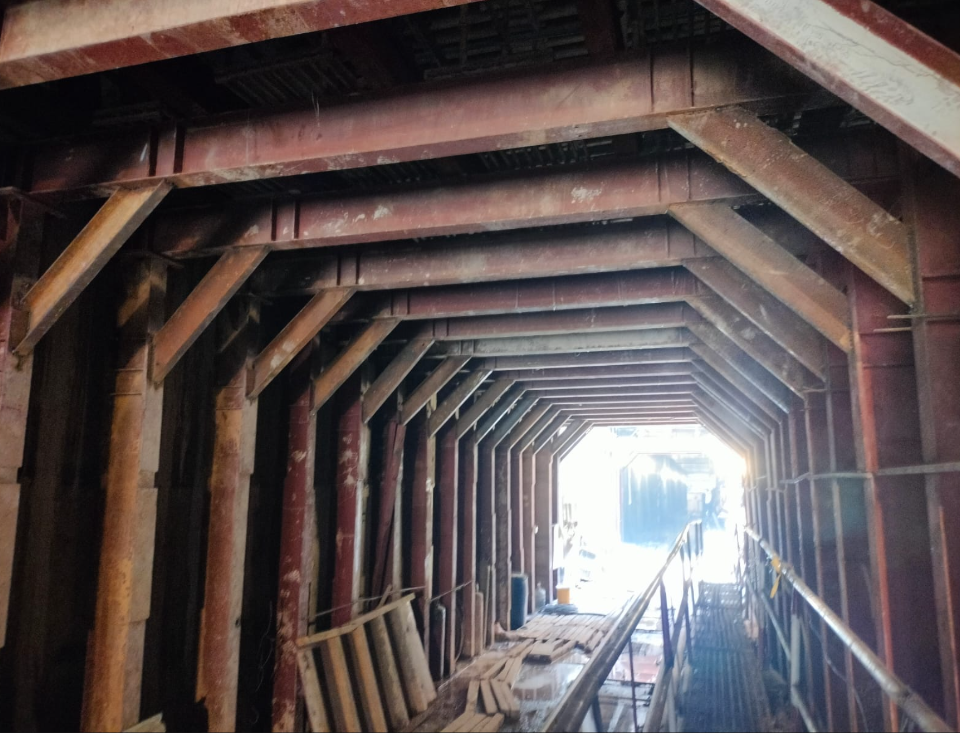
\includegraphics[width=0.85\textwidth]{content/images/strut_interior.png}
    \caption{Interior view of the steel strut frames within the excavation creating a structured temporary support system}
    \label{fig:strut_interior}
\end{figure}

\section{Engineering Challenges}
\par\noindent
The construction of Pulbangash station presents several significant challenges arising from its urban underground setting:

\begin{itemize}
    \item \textbf{Proximity to existing structures} --- Sadar Bazar contains many old buildings with shallow foundations not designed to accommodate ground movements from deep excavation. A comprehensive instrumentation and monitoring programme is essential to protect these structures throughout construction.
    \item \textbf{High water table} --- Delhi's alluvial subsoil contains a significant groundwater table. The D-Wall must maintain watertight panel joints, and dewatering must be carefully controlled to avoid causing settlement outside the construction zone.
    \item \textbf{Utility diversions} --- The area is served by a dense network of utilities --- water mains, sewers, electrical cables, and telecom ducts --- many of which are poorly mapped. Identifying and diverting these without disrupting service is a major logistical challenge.
    \item \textbf{Construction in a live urban environment} --- The surface above remains a functioning road and commercial area throughout construction, requiring careful management of traffic, dust, noise, and public safety.
    \item \textbf{Alignment geometry} --- The unconventional platform layout with part of the platform outside the main box adds complexity to both the structural design and the construction sequencing.
\end{itemize}

\section{Instrumentation and Monitoring}
\par\noindent
Given the sensitive urban environment surrounding the Pulbangash excavation, a comprehensive Instrumentation and Monitoring (I\&M) programme has been implemented by AFCONS Infrastructure Ltd. in accordance with DMRC Method Statement MS/3574/PM/09. The programme provides continuous data on ground movements, structural deformations, and groundwater behaviour throughout construction.

\subsection{Purpose}
\par\noindent
The programme serves three primary purposes. First, \textbf{safety of buildings and utilities} --- by continuously monitoring settlements and lateral movements in the zone of influence, it provides early warning of any excessive ground movement, allowing preventive action well within time. Second, \textbf{design and performance verification} --- monitoring data is compared against design predictions, allowing design assumptions to be refined if actual behaviour deviates significantly. Third, \textbf{construction control} --- parameters such as wall lateral movements, strut loads, and base heave are kept within allowable limits, with construction methodology modified if any trigger level is approached.

\subsection{Settlement Monitoring Points}
\par\noindent
Surface settlement monitoring points (SMPs) are installed around the excavation and above the tunnel alignments to measure ground surface settlements induced by construction activity. Two types are used depending on the ground surface condition.

\par\noindent
\textbf{SMP for Hard Pavement:} Consists of a plastic tapered disc approximately 100 mm in diameter with a retaining nail, installed by drilling a 10 mm diameter hole into the pavement, filling with epoxy, and pressing the disc into position as shown in Figure \ref{fig:smp_pavement}.

\begin{figure}[ht]
    \centering
    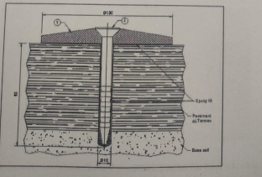
\includegraphics[width=0.6\textwidth]{content/images/smp_pavement.png}
    \caption{Settlement monitoring point installation scheme for hard pavement showing the plastic tapered disc and epoxy nail assembly}
    \label{fig:smp_pavement}
\end{figure}

\par\noindent
\textbf{SMP for Soil:} Consists of a steel survey pin with a hemispherical top, a 16 mm MS extension rod, a protective PVC pipe of 48 mm outer diameter, and a 150 mm grouting plate. Installation requires a 1075 mm deep pit with a concrete pad at the base, assembled and backfilled with compacted fine sand as shown in Figure \ref{fig:smp_soil}.

\begin{figure}[ht]
    \centering
    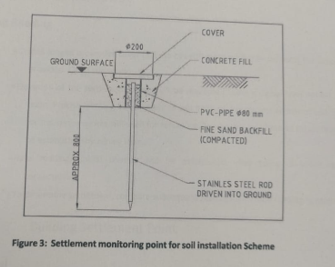
\includegraphics[width=0.6\textwidth]{content/images/smp_soil.png}
    \caption{Settlement monitoring point installation scheme for soil showing the stainless steel rod, PVC pipe, and concrete fill assembly}
    \label{fig:smp_soil}
\end{figure}

\section{TBM and Tunnelling}
\par\noindent
The bored tunnel sections connecting Pulbangash to adjacent stations are constructed using a Tunnel Boring Machine (TBM). Operations are governed by DMRC project specifications and the FHWA Geotechnical Engineering Circulars (GECs), which provide internationally recognised guidance on soft ground tunnelling, subsurface investigation requirements, and TBM operational parameters including face pressure, advance rate, and tail void grouting.

\begin{figure}[ht]
    \centering
    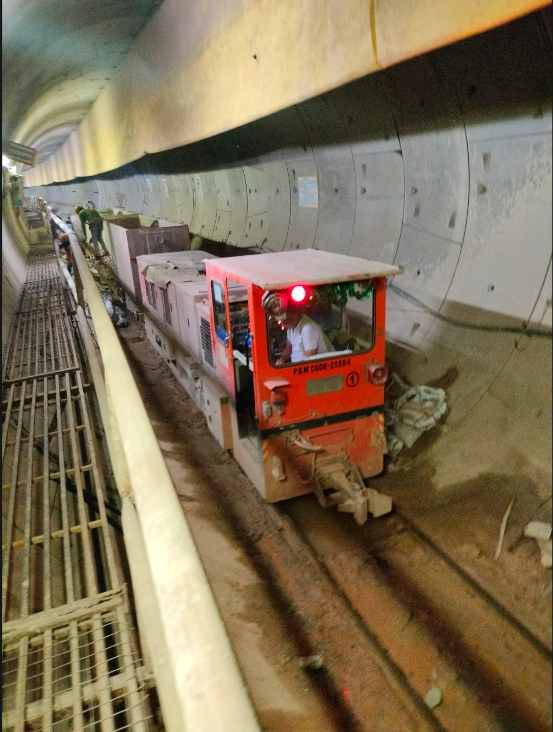
\includegraphics[width=0.85\textwidth]{content/images/tbm_tunnel_loco.png}
    \caption{Battery locomotive inside the completed TBM bored tunnel showing the assembled Universal Tapered Ring lining}
    \label{fig:tbm_tunnel_loco}
\end{figure}

\begin{figure}[ht]
    \centering
    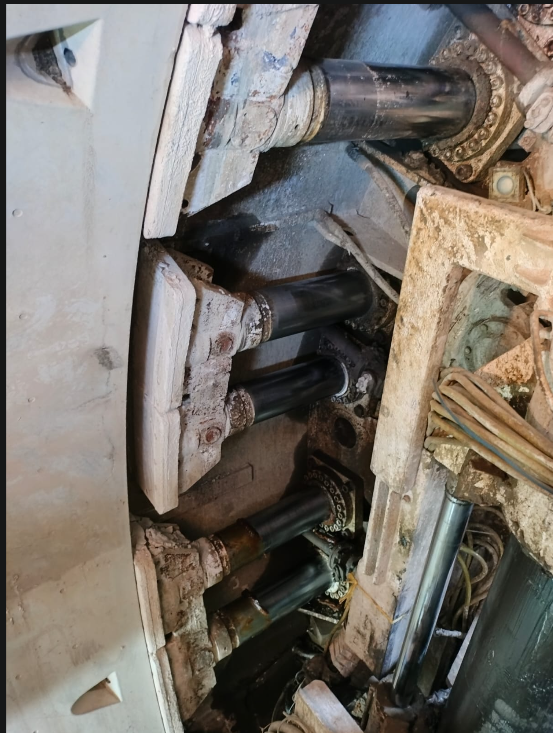
\includegraphics[width=0.75\textwidth]{content/images/tbm_thrust_jacks.png}
    \caption{Closeup of the TBM tail skin showing the hydraulic thrust jacks used to advance the machine against the completed ring lining}
    \label{fig:tbm_thrust_jacks}
\end{figure}

\section{The Soft Eye and TBM Breakthrough}
\par\noindent
The TBM breakthrough --- when the machine exits the running tunnel and enters the station box through the D-Wall --- is one of the highest-risk operations in the construction sequence. To enable passage, a \textbf{Soft Eye} is incorporated into the relevant D-Wall panel, replacing conventional steel rebar with Glass Fibre Reinforced Polymer (GFRP) bars. GFRP provides sufficient structural strength for the D-Wall's temporary retaining function but can be cut through by the TBM cutterhead without damage to the cutting tools. The ground behind the Soft Eye is stabilised using jet grouting or ground freezing before breakthrough, preventing water and soil ingress. The breakthrough requires precise coordination between the TBM operator, site engineer, and the monitoring team watching settlement instruments in real time.

\section{Tunnel Ventilation and MEP Systems}
\par\noindent
An underground metro station requires an integrated set of mechanical, electrical, and plumbing (MEP) systems to provide a safe and comfortable environment for passengers.

\subsection{Tunnel Ventilation System (TVS)}
\par\noindent
The TVS manages airflow through the tunnels and station for both normal operations and emergency scenarios. In normal operations it manages the piston effect created by moving trains, preventing excessive pressure differentials. In emergency mode it switches to smoke extraction, maintaining tenable conditions in escape routes long enough for full passenger evacuation.

\begin{figure}[ht]
    \centering
    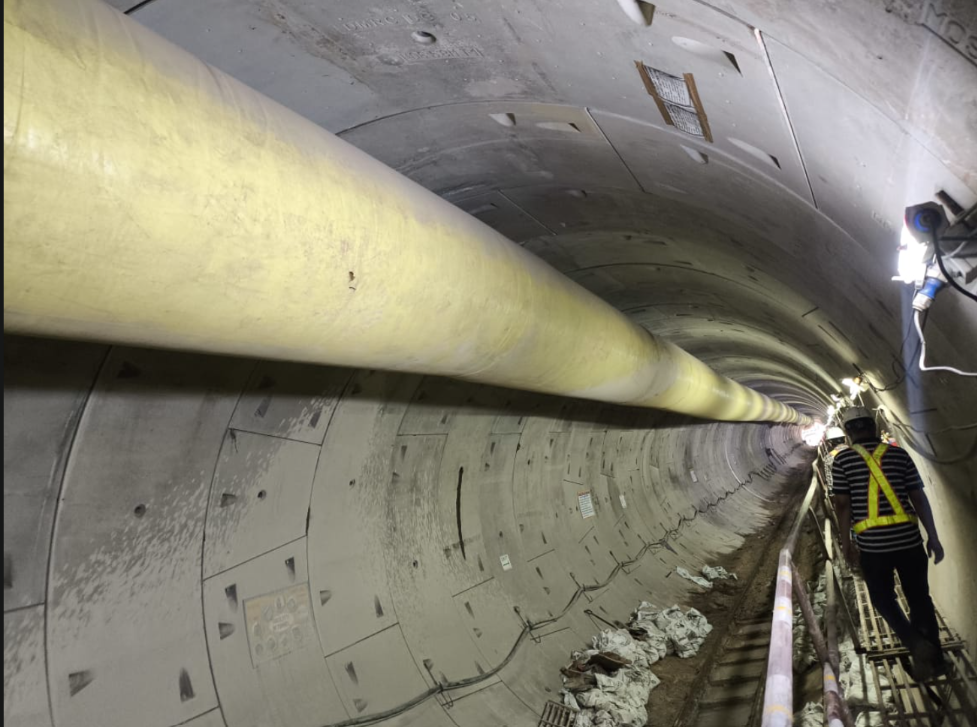
\includegraphics[width=0.85\textwidth]{content/images/tunnel_vent_duct.png}
    \caption{Inside the completed bored tunnel showing the large ventilation duct running along the tunnel crown above the Universal Tapered Ring lining}
    \label{fig:tunnel_vent_duct}
\end{figure}

\begin{figure}[ht]
    \centering
    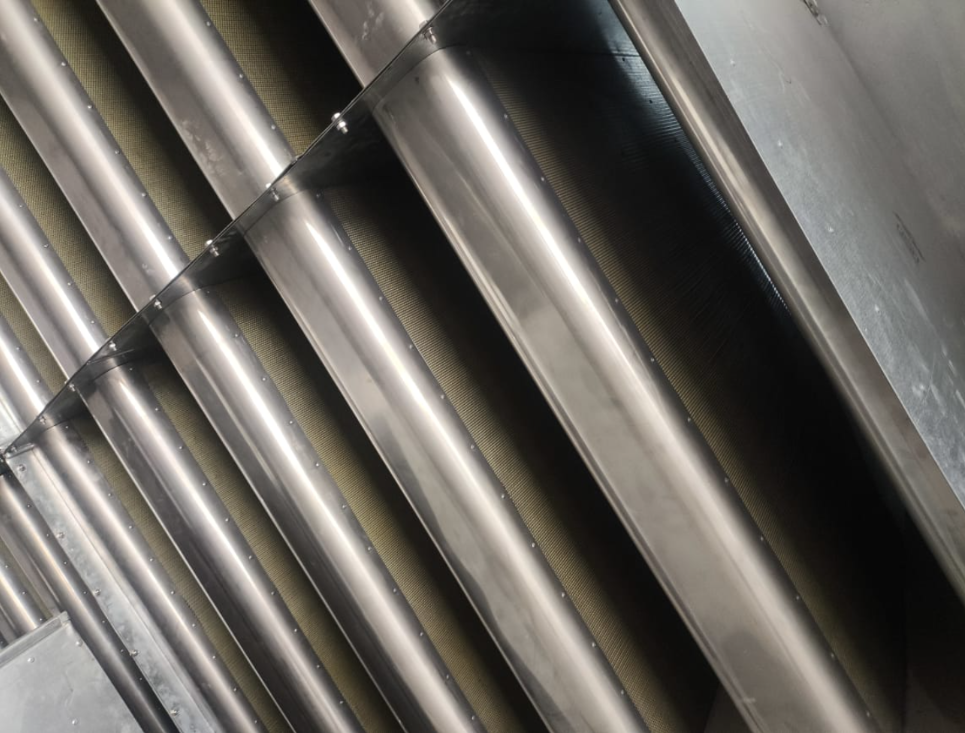
\includegraphics[width=0.75\textwidth]{content/images/station_vent_ducts.png}
    \caption{Stainless steel ventilation ducts inside the station forming part of the Tunnel Ventilation System}
    \label{fig:station_vent_ducts}
\end{figure}

\subsection{Environmental Control System (ECS)}
\par\noindent
The ECS manages the thermal environment within the station using air handling units, chillers, and a network of ducts. Given Delhi's extreme summer temperatures, the cooling load is substantial --- passengers, lighting, equipment, and heat from braking trains all contribute to the internal heat gain the ECS must remove.

\begin{figure}[ht]
    \centering
    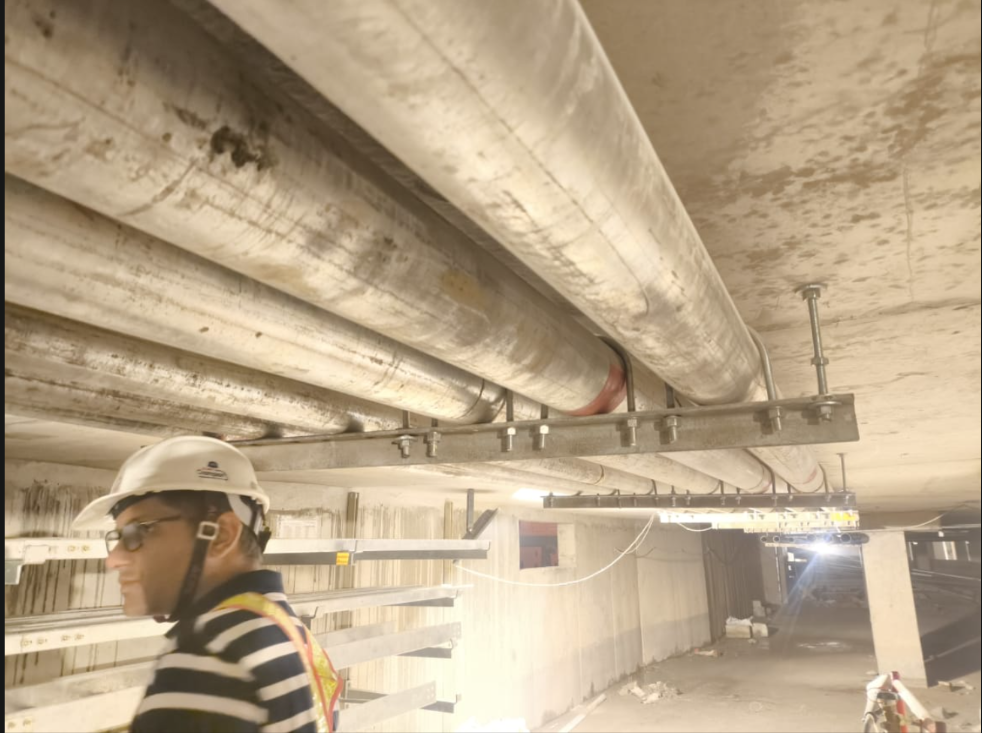
\includegraphics[width=0.85\textwidth]{content/images/mep_pipes.png}
    \caption{Concrete service pipes and ducts running along the station ceiling forming part of the MEP infrastructure}
    \label{fig:mep_pipes}
\end{figure}

\subsection{Platform Screen Doors (PSDs)}
\par\noindent
Platform Screen Doors are full-height glazed barriers separating the platform from the track. They prevent passengers from falling onto the track, significantly improve ECS efficiency by allowing independent air-conditioning of the platform, and reduce noise from passing trains. PSDs are interlocked with train doors, opening only when a train is correctly stopped and aligned at the platform.

\section{Station Rooms and Their Uses}
\par\noindent
The station box accommodates numerous ancillary rooms essential to operations. During the site visit, several of these rooms were observed in various stages of completion, as seen in Figure \ref{fig:station_manager_room}.

\begin{figure}[ht]
    \centering
    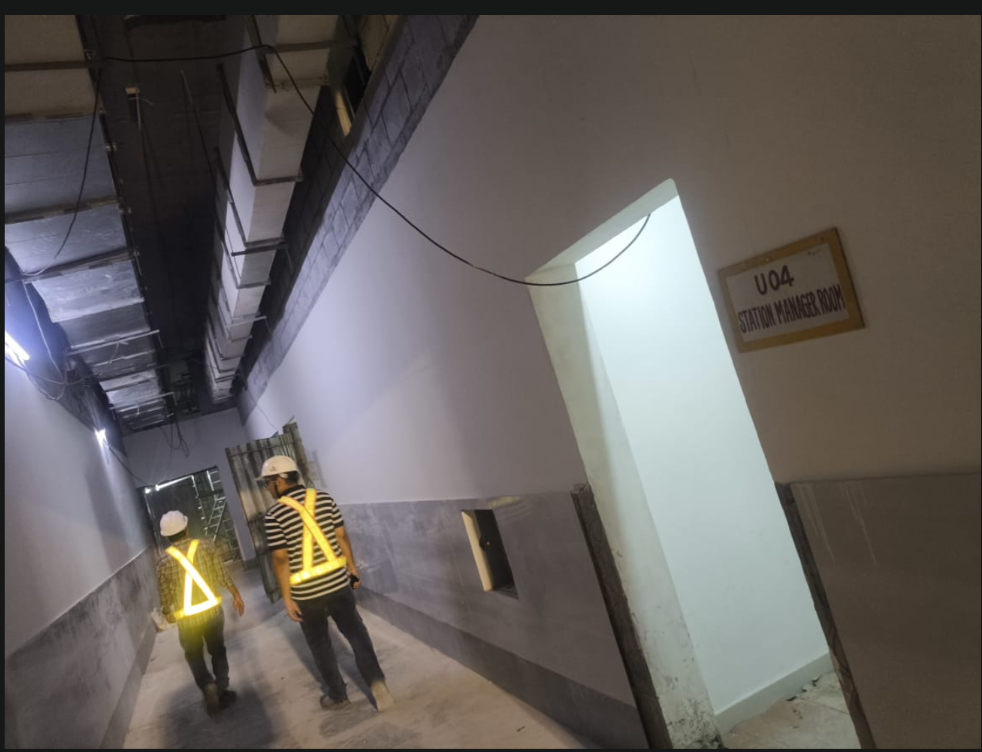
\includegraphics[width=0.85\textwidth]{content/images/station_manager_room.png}
    \caption{Station Manager Room (U04) signage visible in a finished corridor at Pulbangash station}
    \label{fig:station_manager_room}
\end{figure}

\par\noindent
The key rooms include:
\begin{itemize}
    \item \textbf{Station Controller Room} --- The nerve centre of station operations, housing SCADA workstations monitoring all station systems.
    \item \textbf{Traction Substation} --- Converts incoming high-voltage AC grid power to the DC traction voltage required by trains.
    \item \textbf{Auxiliary Equipment Room (AER)} --- Contains switchgear and distribution boards for the station's own electrical supply.
    \item \textbf{Relay/Signal Equipment Room} --- Houses signalling and communications equipment including ATP and ATO systems.
    \item \textbf{UPS Room} --- Maintains critical systems during power failure including communications, fire detection, and emergency lighting.
    \item \textbf{Pump Room} --- Houses sump pumps removing groundwater infiltration and drainage from within the station box.
\end{itemize}

\section{Fire Safety and Emergency Egress}
\par\noindent
Fire safety provisions at Pulbangash include multiple emergency exit staircases at regular intervals along the platform and concourse, each leading to an independent surface exit so that no single fire can block all escape routes simultaneously. Emergency lighting on dedicated UPS circuits illuminates escape routes during power failure. The TVS smoke extraction mode maintains tenable conditions during evacuation. Dry riser systems, fire hose reels, and hydrant points are distributed throughout the station, with fire detection by smoke and heat detectors connected to the station controller's SCADA system.

\section{Fit-Out, Integration, and Testing}
\par\noindent
Once the civil structure is watertight and structurally complete, the station enters the fit-out phase --- architectural finishes, MEP systems, PSDs, escalators, lifts, and communications infrastructure are all installed. Integration and testing follows, during which all systems are tested together as an integrated whole including trial train runs, PSD interlock testing, evacuation drills, and commissioning of all traction and signalling systems. Only after successful integrated testing and a safety audit by the Commissioner of Metro Rail Safety (CMRS) is the station certified for revenue operations.

\section{Maintenance and Allied Services}
\par\noindent
Long-term performance of the station depends on a structured maintenance regime. The civil structure requires periodic inspection of the D-Wall and base slab for water ingress, cracking, or carbonation. Mechanical systems --- ventilation fans, chillers, escalators, lifts, and PSDs --- require scheduled preventive maintenance alongside reactive maintenance capability. Traction and signalling systems are maintained by DMRC's operations team under strict maintenance windows during non-operational hours to avoid any disruption to revenue service.